\documentclass[11pt,a4paper]{article}
% ---------------------------------------------------------------------
%  TFPT --- The frontier items: eta_B, m_p/m_e, Koide, dark matter, quantum gravity
%  Honest status: the genuine handle, the precision, and what is NOT a clean ladder.
%  No fabricated compiler rungs.  All numbers machine-verified.
% ---------------------------------------------------------------------
\usepackage[T1]{fontenc}
\usepackage[utf8]{inputenc}
\usepackage[english]{babel}
\usepackage{lmodern}
\usepackage[a4paper,margin=2.3cm]{geometry}
\usepackage{amsmath,amssymb}
\usepackage{booktabs,array,tabularx}
\usepackage{enumitem}
\usepackage{xcolor}
\usepackage{tikz}
\usetikzlibrary{positioning,arrows.meta}
\usepackage[most]{tcolorbox}
\usepackage{microtype}
\usepackage[hidelinks,colorlinks=true,linkcolor=blue!55!black,urlcolor=blue!55!black]{hyperref}
\emergencystretch=3em

% ---------------------------------------------------------------------
%  tfpt_style.tex -- THE shared visual style for every TFPT document.
%  Single source for colours, status markers, marker key, the \veri
%  script reference, the tcolorbox families, and the running
%  header/footer.  \input AFTER xcolor + tcolorbox[most] + hyperref are
%  loaded (every paper loads those).  Each document sets its short
%  running title before \begin{document}, e.g.
%        \def\TFPTdoctitle{Architecture and the E8 Compiler}
%  ---------------------------------------------------------------------
\usepackage{fancyhdr}
\usepackage{etoolbox}
\usepackage{tikz}
\usetikzlibrary{positioning,arrows.meta,fit,backgrounds,calc,shapes.geometric,shapes.misc}

% ---- single-source author / version / automatic date stamp ----
% ---------------------------------------------------------------------
%  tex-artefacts/version.tex -- single source for author list, version
%  and the automatic title-page date stamp of every TFPT document.
%  \input by tex-artefacts/tfpt_style.tex, so every paper that loads the
%  shared style automatically gets:
%     \TFPTauthors   -- the author list (use as \author{\TFPTauthors})
%     \TFPTversion   -- curated semantic version (bump per release; mirror
%                       the bump in changelog.tex)
%     \TFPTrev       -- auto build revision = git commit count, injected by
%                       build.sh into tex-artefacts/version-auto.tex
%                       (gitignored); falls back to "dev" for standalone runs
%     \TFPTdatestamp -- the title-page date line: \today + version + revision
%  build.sh also writes tex-artefacts/release-version.txt (gitignored):
%     "{TFPTversion} (rev {git commit count})" for Zenodo + release tooling.
%  Bump \TFPTversion here ONCE; it then updates in all papers at the next build.
% ---------------------------------------------------------------------
\def\TFPTauthors{Stefan Hamann \and Alessandro Rizzo}
\def\TFPTversion{5.3}
\def\TFPTrev{dev}
% build.sh regenerates the line below with the live git commit count:
\InputIfFileExists{tex-artefacts/version-auto.tex}{}{}
\def\TFPTdatestamp{\today\,\textperiodcentered\,v\TFPTversion\,(rev~\TFPTrev)}


% ---- colours (canonical TFPT palette) ----
\definecolor{tfblue}{HTML}{1F4E79}
\definecolor{tfgreen}{HTML}{1E7B45}
\definecolor{tfred}{HTML}{9B2226}
\definecolor{tfgold}{HTML}{B8860B}
\definecolor{tfgray}{HTML}{555555}

% ---- status markers (simplified 4-class display system) ----
% Reader-facing markers collapse to FOUR classes.  The fine-grained per-claim
% type (Axiom / Formal / Lattice / Numerical / Identity / Physical) stays in
% verification/status_ledger.csv -- the single source of truth -- so no fidelity
% is lost; the papers just show the coarse class so a reader is not overwhelmed.
%   [E] exact / machine-proven  (identity, Lie/lattice, formalised, numerical FP)
%   [C] conditional             (physical / bridge / readout, under named hypotheses)
%   [O] open / axiom            (declared input or genuine gap)
%   [X] kill test               (falsifiable threshold)
\newcommand{\mE}{{\small\textcolor{tfgreen!70!black}{\textbf{[E]}}}}
\newcommand{\mC}{{\small\textcolor{tfgold!78!black}{\textbf{[C]}}}}
\newcommand{\mO}{{\small\textcolor{tfred!80!black}{\textbf{[O]}}}}
\newcommand{\mX}{{\small\textcolor{tfred!58!black}{\textbf{[X]}}}}
% backward-compatible aliases: the old fine-grained names now render their class,
% so any not-yet-rewritten call site (or the standalone changelog) still compiles.
\newcommand{\tI}{\mE}\newcommand{\tL}{\mE}\newcommand{\tF}{\mE}\newcommand{\tN}{\mE}
\newcommand{\tIalg}{\mE}\newcommand{\tInum}{\mE}
\newcommand{\tP}{\mC}\newcommand{\tB}{\mC}\newcommand{\tR}{\mC}
\newcommand{\tA}{\mO}
\newcommand{\tX}{\mX}

% compact marker legend, placed under a marker-bearing table
\newcommand{\markerkey}{\par\vspace{1.5pt}\noindent{\scriptsize\itshape
  \textcolor{black!58}{Marker key:\ \mE~exact / machine-proven\,$\cdot$\,%
  \mC~conditional (holds under named hypotheses)\,$\cdot$\,%
  \mO~open / axiom\,$\cdot$\,\mX~falsifiable kill test.\ \
  Per-claim fine type in \texttt{verification/status\_ledger.csv}.}}\par\vspace{2pt}}

% horizontal badge bar (place once near the front of a document)
\newcommand{\TFPTbadges}{\par\noindent
  \fcolorbox{tfgreen!55!black}{tfgreen!8}{\scriptsize\mE\,exact / machine-proven}\hfill
  \fcolorbox{tfgold!70!black}{tfgold!10}{\scriptsize\mC\,conditional}\hfill
  \fcolorbox{tfred!75!black}{tfred!8}{\scriptsize\mO\,open / axiom}\hfill
  \fcolorbox{tfred!60!black}{tfred!6}{\scriptsize\mX\,kill test}\par\vspace{3pt}}

% inline reference to the script that machine-checks a claim (see verification/)
\newcommand{\veri}[1]{\,{\footnotesize\textcolor{tfblue!70!black}{[\,\texttt{verification/#1}\,]}}}
% lightweight inline colour-mark for a bare verification-script token in running
% prose / tables, e.g. \vref{v108}, \vref{v49}/\vref{v71}.  Same blue as \veri so a
% reader instantly sees "this is a machine-checked module reference".
\newcommand{\vref}[1]{\textcolor{tfblue!72!black}{\textsf{#1}}}

% ---- tcolorbox families (one visual language across all documents) ----
% keybox  : the central claim / reading of a section (blue)
% winbox  : an established result / closure (green)
% gapbox  : an open gate / honest caveat / kill criterion (red)
% auditbox: a recorded audit fingerprint, not load-bearing (gold)
% navbox  : a light, neutral navigation / reference card (document map, etc.)
% Visual language (deliberately light): a faint tint, a thin coloured frame
% and a light title band with dark coloured title text -- NOT a heavy
% white-on-saturated-colour bar -- so a page never reads as a wall of boxes.
\newtcolorbox{keybox}[1][]{enhanced,breakable,boxrule=0.5pt,arc=1.5pt,
  colback=tfblue!4!white,colframe=tfblue!70!black,coltitle=tfblue!88!black,colbacktitle=tfblue!12!white,
  fonttitle=\bfseries\small,fontupper=\small,title={#1},left=2mm,right=2mm,top=1mm,bottom=1mm}
% non-breaking variant (front-matter cards that should never split across a page)
\newtcolorbox{keyboxnb}[1][]{enhanced,breakable=false,boxrule=0.5pt,arc=1.5pt,
  colback=tfblue!4!white,colframe=tfblue!70!black,coltitle=tfblue!88!black,colbacktitle=tfblue!12!white,
  fonttitle=\bfseries\small,fontupper=\small,title={#1},left=2mm,right=2mm,top=1mm,bottom=1mm}
\newtcolorbox{winbox}[1][]{enhanced,breakable,boxrule=0.5pt,arc=1.5pt,
  colback=tfgreen!5!white,colframe=tfgreen!65!black,coltitle=tfgreen!50!black,colbacktitle=tfgreen!14!white,
  fonttitle=\bfseries\small,fontupper=\small,title={#1},left=2mm,right=2mm,top=1mm,bottom=1mm}
\newtcolorbox{gapbox}[1][]{enhanced,breakable,boxrule=0.5pt,arc=1.5pt,
  colback=tfred!4!white,colframe=tfred!70!black,coltitle=tfred!75!black,colbacktitle=tfred!12!white,
  fonttitle=\bfseries\small,fontupper=\small,title={#1},left=2mm,right=2mm,top=1mm,bottom=1mm}
% non-breaking variants (callouts that must stay whole on one page, embedded in text)
\newtcolorbox{winboxnb}[1][]{enhanced,breakable=false,boxrule=0.5pt,arc=1.5pt,
  colback=tfgreen!5!white,colframe=tfgreen!65!black,coltitle=tfgreen!50!black,colbacktitle=tfgreen!14!white,
  fonttitle=\bfseries\small,fontupper=\small,title={#1},left=2mm,right=2mm,top=1mm,bottom=1mm}
\newtcolorbox{gapboxnb}[1][]{enhanced,breakable=false,boxrule=0.5pt,arc=1.5pt,
  colback=tfred!4!white,colframe=tfred!70!black,coltitle=tfred!75!black,colbacktitle=tfred!12!white,
  fonttitle=\bfseries\small,fontupper=\small,title={#1},left=2mm,right=2mm,top=1mm,bottom=1mm}
\newtcolorbox{auditbox}[1][]{enhanced,breakable,boxrule=0.5pt,arc=1.5pt,
  colback=tfgold!7!white,colframe=tfgold!70!black,coltitle=tfgold!45!black,colbacktitle=tfgold!16!white,
  fonttitle=\bfseries\small,fontupper=\small,title={#1},left=2mm,right=2mm,top=1mm,bottom=1mm}
\newtcolorbox{navbox}[1][]{enhanced,breakable,boxrule=0.5pt,arc=1.5pt,
  colback=tfgray!3!white,colframe=tfgray!55,coltitle=tfgray!30!black,colbacktitle=tfgray!12!white,
  fonttitle=\bfseries\small,fontupper=\small,title={#1},left=2mm,right=2mm,top=1mm,bottom=1mm}
% back-compatibility aliases (older box names map onto the canonical types)
\newtcolorbox{audbox}[1][]{enhanced,breakable,boxrule=0.5pt,arc=1.5pt,
  colback=tfgold!7!white,colframe=tfgold!70!black,coltitle=tfgold!45!black,colbacktitle=tfgold!16!white,
  fonttitle=\bfseries\small,fontupper=\small,title={#1},left=2mm,right=2mm,top=1mm,bottom=1mm}
\newtcolorbox{resbox}[1][]{enhanced,breakable,boxrule=0.5pt,arc=1.5pt,
  colback=tfgreen!5!white,colframe=tfgreen!55!black,coltitle=tfgreen!50!black,colbacktitle=tfgreen!12!white,
  fonttitle=\bfseries\small,fontupper=\small,title={#1},left=2mm,right=2mm,top=1mm,bottom=1mm}
\newtcolorbox{roadbox}[1][]{enhanced,breakable,boxrule=0.5pt,arc=1.5pt,
  colback=tfgreen!5!white,colframe=tfgreen!55!black,coltitle=tfgreen!50!black,colbacktitle=tfgreen!12!white,
  fonttitle=\bfseries\small,fontupper=\small,title={#1},left=2mm,right=2mm,top=1mm,bottom=1mm}
\newtcolorbox{intbox}[1][]{enhanced,breakable,boxrule=0.5pt,arc=1.5pt,
  colback=tfgold!7!white,colframe=tfgold!70!black,coltitle=tfgold!45!black,colbacktitle=tfgold!16!white,
  fonttitle=\bfseries\small,fontupper=\small,title={#1},left=2mm,right=2mm,top=1mm,bottom=1mm}

% ---- colour-marked display formula (load-bearing key equations) ----
% A highlighted formula line: a coloured left accent bar + faint tint, no full
% frame -- so a key equation is visually set apart from the running prose
% without becoming yet another box.  Use:  \begin{keyeq}$\displaystyle ...$\end{keyeq}
\newtcolorbox{keyeq}{blanker,breakable=false,halign=center,
  colback=tfgold!8!white,borderline west={2.4pt}{0pt}{tfgold!75!black},
  left=8pt,right=6pt,top=3pt,bottom=3pt,before skip=5pt,after skip=5pt}

% ---- running header / footer (consistent across all documents) ----
\providecommand{\TFPTdoctitle}{}
\setlength{\headheight}{14pt}
\pagestyle{fancy}
\fancyhf{}
\fancyhead[L]{\footnotesize\textcolor{tfgray}{\textit{TFPT}\,\textbullet\,\TFPTdoctitle}}
\fancyhead[R]{\footnotesize\textcolor{tfgray}{\thepage}}
\fancyfoot[L]{\scriptsize\textcolor{tfgray}{v\TFPTversion\,\textperiodcentered\,rev~\TFPTrev}}
\renewcommand{\headrulewidth}{0.3pt}
\renewcommand{\footrulewidth}{0pt}
\fancypagestyle{plain}{\fancyhf{}\renewcommand{\headrulewidth}{0pt}%
  \fancyfoot[C]{\footnotesize\textcolor{tfgray}{\thepage}}%
  \fancyfoot[L]{\scriptsize\textcolor{tfgray}{v\TFPTversion\,\textperiodcentered\,rev~\TFPTrev}}}

% ---- shared figure macros (claim stack, anchor cockpit, E8 glue, 2/3 motif, K5) ----
%  (this fragment lives in tex-artefacts/ and is \input by documents compiled from
%   the repository root, so the path is given relative to that root.)
% ---------------------------------------------------------------------
%  tfpt_figures.tex -- shared, reusable TikZ figure macros for every
%  TFPT document.  \input by tfpt_style.tex (which loads tikz + the
%  needed libraries + etoolbox).  Each macro draws a self-contained
%  centred figure; nothing is drawn until the macro is called.
%
%    \TFPTclaimstack[zone]  -- the architecture claim stack (B3); the
%                              optional zone in {axioms,anchor,compiler,
%                              sm,bridges,frontier} is highlighted.
%    \TFPTanchorcockpit      -- the anchor a=(1,1,2) cockpit (B4)
%    \TFPTeightglue          -- the D5 (+) A3 +mu4 => E8 glue (B5)
%    \TFPTmotif              -- the 2/3 motif map (B6)
%    \TFPTactionkfive        -- the K5 action-lattice mnemonic (B7)
% ---------------------------------------------------------------------

% ===== B3: the architecture claim stack =========================
\newcommand{\tfhl}[1]{\ifdefstring{\tfcur}{#1}{cbhi}{cbnl}}
\newcommand{\TFPTclaimstack}[1][none]{%
\def\tfcur{#1}%
\begin{center}
\begin{tikzpicture}[font=\footnotesize,
  cb/.style={rounded corners=2pt,inner sep=4pt,text width=118mm,align=center,minimum height=8.5mm},
  cbnl/.style={line width=0.5pt}, cbhi/.style={line width=1.5pt},
  ar/.style={-{Stealth[length=2.2mm]},tfgray,semithick}]
  \node[cb,fill=tfred!8,draw=tfred!75!black,\tfhl{axioms}] (axioms)
    {\textbf{P1}\,$c_3=\tfrac1{8\pi}$ \quad \textbf{P2}\,$g_{\mathrm{car}}=5$ \ \textcolor{tfgray}{\itshape(two inputs, [O] axioms)}};
  \node[cb,fill=tfblue!8,draw=tfblue,\tfhl{anchor},below=3.5mm of axioms] (anchor)
    {Anchor $a=(1,1,2)$:\ $e_1,e_2,e_3=4,5,2$ \ \textcolor{tfgray}{\itshape([E] exact)}};
  \node[cb,fill=tfgreen!10,draw=tfgreen!70!black,\tfhl{compiler},below=3.5mm of anchor] (compiler)
    {Discrete compiler:\ $D_5\oplus A_3+\mu_4\Rightarrow E_8$,\ $h=30$,\ $\varphi_0$ \ \textcolor{tfgray}{\itshape([E] exact)}};
  \node[cb,fill=tfgreen!7,draw=tfgreen!60!black,\tfhl{sm},below=3.5mm of compiler] (sm)
    {SM skeleton:\ three families, hypercharges, flavor matrix $R$ \ \textcolor{tfgray}{\itshape([E])}};
  \node[cb,fill=tfgold!12,draw=tfgold!80!black,\tfhl{bridges},below=3.5mm of sm] (bridges)
    {Physical bridges:\ $v_{\mathrm{geo}}$,\ $G_{\mathrm{net}}$,\ $F_{\mathrm{transfer}}$ \ \textcolor{tfgray}{\itshape([C] bridges)}};
  \node[cb,fill=tfgray!12,draw=tfgray!70!black,\tfhl{frontier},below=3.5mm of bridges] (frontier)
    {Frontier readouts:\ $\Lambda$, inflation, $\eta_B$, dark matter, QG \ \textcolor{tfgray}{\itshape([C]/[O])}};
  \draw[ar] (axioms)--(anchor); \draw[ar] (anchor)--(compiler);
  \draw[ar] (compiler)--(sm);   \draw[ar] (sm)--(bridges); \draw[ar] (bridges)--(frontier);
\end{tikzpicture}
\end{center}}

% ===== B4: the anchor cockpit ====================================
\newcommand{\TFPTanchorcockpit}{%
\begin{center}
\begin{tikzpicture}[font=\footnotesize,
  pan/.style={rounded corners=2pt,draw=tfblue!60,fill=tfblue!4,inner sep=5pt,
    text width=46mm,align=left},
  hd/.style={font=\bfseries\small,tfblue}]
  \node[pan] (e) {\textbf{elementary} $e_k(a)$\\[2pt]
     $e_1=4\to|\mu_4|$\\ $e_2=5\to g_{\mathrm{car}}$\\ $e_3=2\to|\mathbb Z_2|$\\[2pt]
     $c_3=\tfrac1{2e_1\pi}=\tfrac1{8\pi}$};
  \node[pan,right=4mm of e] (p) {\textbf{power sums} $p_n=2+2^n$\\[2pt]
     $p_0,p_1,p_2,p_3=3,4,6,10$\\ $p_1p_2p_3=240=|R(E_8)|$\\ $p_4-p_3=8=\operatorname{rank}E_8$\\
     $\Rightarrow\dim E_8=248$};
  \node[pan,right=4mm of p] (m) {\textbf{derived motifs}\\[2pt]
     $4,5,8,16,25,$\\ $30,41,120,240$\\[2pt]
     \textcolor{tfgray}{\itshape one anchor,}\\ \textcolor{tfgray}{\itshape many projections}};
  \node[hd,above=1mm of p.north] {$a=(1,1,2)$ \ \textcolor{tfgray}{\footnotesize\itshape[E]}};
\end{tikzpicture}
\end{center}}

% ===== B5: the E8 glue ===========================================
\newcommand{\TFPTeightglue}{%
\begin{center}
\begin{tikzpicture}[font=\footnotesize,
  d/.style={rounded corners=2pt,draw=tfblue,fill=tfblue!6,inner sep=4pt,align=center,text width=36mm},
  mid/.style={rounded corners=2pt,draw=tfgold!80!black,fill=tfgold!12,inner sep=4pt,align=center,text width=52mm},
  e8/.style={rounded corners=2pt,draw=tfgreen!70!black,fill=tfgreen!10,inner sep=4pt,align=center,text width=52mm,font=\bfseries},
  rt/.style={rounded corners=2pt,draw=tfgreen!55!black,fill=tfgreen!6,inner sep=3pt,align=center,text width=52mm},
  side/.style={rounded corners=2pt,draw=tfgray!55,fill=tfgray!6,inner sep=4pt,align=left,text width=34mm,font=\scriptsize},
  ar/.style={-{Stealth[length=2mm]},tfgray,semithick}]
  \node[d] (d5) {$D_5$ discriminant\\ $\mathbb Z_4$, $q=5/4$};
  \node[d,right=10mm of d5] (a3) {$A_3$ discriminant\\ $\mathbb Z_4$, $q=3/4$};
  \node[mid,below=5mm of $(d5)!0.5!(a3)$] (glue) {$\mu_4$ anti-isometry\ ($q$-sum $=2$)};
  \node[e8,below=4mm of glue] (e8) {even unimodular $E_8$ lattice};
  \node[rt,below=4mm of e8] (rt) {$240$ roots,\ rank $8$,\ $\dim=248$};
  \node[side,right=8mm of glue] (why) {\textbf{why unique?}\\ rank $8$\\ even\\ unimodular\\ positive definite};
  \draw[ar] (d5)--(glue); \draw[ar] (a3)--(glue);
  \draw[ar] (glue)--(e8); \draw[ar] (e8)--(rt);
\end{tikzpicture}\\[2pt]
{\scriptsize\itshape $D_5\oplus A_3+\mu_4\Rightarrow E_8$ --- the unique even unimodular rank-$8$ glue \ [E] exact (lattice).}
\end{center}}

% ===== B5b: the double pushout (one glue, two categories) ========
\newcommand{\TFPTdoublepushout}{%
\begin{center}
\begin{tikzpicture}[font=\footnotesize,>={Stealth[length=2mm]},
  lat/.style={rounded corners=2pt,draw=tfblue,fill=tfblue!6,inner sep=5pt,align=center,text width=34mm},
  net/.style={rounded corners=2pt,draw=tfblue!70!black,fill=tfblue!4,inner sep=5pt,align=center,text width=34mm},
  e8l/.style={rounded corners=2pt,draw=tfgold!80!black,fill=tfgold!12,inner sep=5pt,align=center,text width=34mm,font=\bfseries},
  e8n/.style={rounded corners=2pt,draw=tfgreen!70!black,fill=tfgreen!10,inner sep=5pt,align=center,text width=34mm,font=\bfseries},
  ar/.style={->,tfgray,semithick},
  lb/.style={font=\scriptsize,text=black,align=center,fill=white,inner sep=1.5pt}]
  \node[lat] (LL) at (0,2.5)   {$D_5\oplus A_3$\\[1pt]\scriptsize root lattices,\ $\mathrm{disc}=\Z_4$};
  \node[e8l] (LR) at (6.6,2.5) {$E_8$\\[1pt]\scriptsize even unimodular,\ $\det 1$};
  \node[net] (BL) at (0,0)     {$(D_5)_1\otimes(A_3)_1$\\[1pt]\scriptsize chiral nets,\ $c=8$};
  \node[e8n] (BR) at (6.6,0)   {$(E_8)_1$\\[1pt]\scriptsize holomorphic,\ $\mu$-index $1$};
  \draw[ar] (LL)--node[lb]{$+\,\mu_4$ glue}(LR);
  \draw[ar] (BL)--node[lb]{$\rtimes\,\mu_4$ extension}(BR);
  \draw[ar] (LL)--node[lb,left=-1pt]{level-$1$}(BL);
  \draw[ar] (LR)--node[lb,right=-1pt]{level-$1$}(BR);
\end{tikzpicture}\\[2pt]
{\scriptsize\itshape One operation, two categories: the order-$|\mu_4|{=}4$ glue is the lattice pushout
$D_5\oplus A_3+\mu_4\Rightarrow E_8$ \emph{and} the simple-current / anyon-condensation extension
$(D_5)_1\otimes(A_3)_1\rtimes\mu_4\cong(E_8)_1$; the square commutes. \ [E] exact.}
\end{center}}

% ===== B6: the 2/3 motif map =====================================
\newcommand{\TFPTmotif}{%
\begin{center}
\begin{tikzpicture}[font=\footnotesize,
  ex/.style={rounded corners=2pt,draw=tfgreen!70!black,fill=tfgreen!8,inner sep=4pt,align=center,text width=92mm},
  br/.style={rounded corners=2pt,draw=tfgold!80!black,fill=tfgold!12,inner sep=4pt,align=center,text width=92mm},
  ar/.style={-{Stealth[length=2mm]},tfgray,semithick}]
  \node[ex] (a) {$|\mathbb Z_2|/N_{\mathrm{fam}}=2/3$ \ \textcolor{tfgray}{\itshape(anchor ratio)}};
  \node[ex,below=3mm of a] (b) {parabolic weights $\{0,\tfrac13,\tfrac23\}=\operatorname{spec}A_0^\star$};
  \node[ex,below=3mm of b] (c) {transfer spectrum $\{1,(2/3)^6,(1/3)^6\}$,\ gap $6\log\tfrac32$};
  \node[br,below=3mm of c] (d) {Koide target $2/3$ \ \textcolor{tfgray}{\itshape(source$\to$pole bridge [C])}};
  \node[br,below=3mm of d] (e) {Nariai / horizon entropy bound $2/3$ \ \textcolor{tfgray}{\itshape([C])}};
  \draw[ar] (a)--(b); \draw[ar] (b)--(c); \draw[ar] (c)--(d); \draw[ar] (d)--(e);
\end{tikzpicture}\\[2pt]
{\scriptsize\itshape Green: exact motif ([E]).\quad Gold: physical bridge ([C]) --- the same ratio, two epistemic types.}
\end{center}}

% ===== B7: the K5 action-lattice mnemonic ========================
%  Layout: complete graph K5 (pentagon, all 10 edges) on the LEFT, the
%  Pascal-row reading list on the RIGHT, vertically centred on the graph
%  so the two blocks never overlap.
\newcommand{\TFPTactionkfive}{%
\begin{center}
\begin{tikzpicture}[font=\scriptsize]
  % --- K5 vertices on a regular pentagon, centred at the origin ---
  \foreach \i in {1,...,5}{\coordinate (k\i) at ({90+72*(\i-1)}:12mm);}
  \begin{scope}[on background layer]
    \foreach \i in {1,...,5}{\foreach \j in {1,...,5}{\ifnum\i<\j
      \draw[tfgray!55,line width=0.5pt] (k\i)--(k\j);\fi}}
  \end{scope}
  \foreach \i in {1,...,5}{\fill[tfblue!70!black] (k\i) circle (1.8pt);}
  \node[tfgray,font=\scriptsize\itshape] at (0,-1.9) {$K_5$};
  % --- reading list, anchored to the right of the whole graph, centred ---
  \node[anchor=west,align=left,inner sep=0pt] at (1.9cm,0) {%
    $\tbinom51=5$\ \ vertices --- action $x^1$ (Hubble slot)\\[1pt]
    $\tbinom52=10$\ edges --- $\Lambda$ density pair $x^{10}$\\[1pt]
    $\tbinom53=10$\ triangles --- dual sector\\[1pt]
    $\tbinom54=5$\ \ complements --- inverse sector\\[1pt]
    $\tbinom55=1$\ \ determinant --- closure};
\end{tikzpicture}\\[2pt]
{\scriptsize\itshape $K_5$ on the five carrier slots; the action powers $x^{1},x^{5},x^{10}$ are its
$\tbinom5k$ faces \ \textcolor{tfgray}{(mnemonic; the physical scale map stays [C]).}}
\end{center}}


\newcommand{\phiz}{\varphi_0^{\mathrm{ret}}}
\newcommand{\cthree}{c_3}
\newcommand{\Mpl}{M_{\mathrm{Pl}}}
\newcommand{\Nfam}{N_{\mathrm{fam}}}
\newcommand{\Z}{\mathbb{Z}}
\setlist{itemsep=2pt,topsep=3pt}
\newcolumntype{Y}{>{\raggedright\arraybackslash}X}

\title{\vspace{-1.2cm}\textbf{TFPT --- Frontier items}\\[2mm]
\large $\eta_B$, $m_p/m_e$, the Koide relation, dark matter and quantum gravity ---\\
the honest status, not forced onto the ladder}
\author{\TFPTauthors}\date{\TFPTdatestamp}

\def\TFPTdoctitle{Frontier}
\begin{document}
\maketitle
\vspace{-0.6cm}

\begin{keybox}[What this document is about --- the status authority for the frontier]
The honest frontier: which physics has a genuine TFPT handle and which does not. For each of
$\eta_B$, $m_p/m_e$, the Koide relation, dark matter and full quantum gravity, this note states the
genuine structural handle, the precision with which it currently lands, and --- crucially --- what is
\emph{not} a clean compiler power and is deliberately \emph{not} forced onto the ladder. \textbf{This
document is the status authority for the frontier items:} where any other document's wording and the
markers here disagree, the typing here (and the \texttt{status\_ledger.csv}) wins.
\end{keybox}

% ---------------------------------------------------------------------
%  tfpt_docset.tex -- THE canonical TFPT document-set box.
%  Single source of truth for the document list; \input by the
%  introduction and every paper. Uses only universally available
%  macros (keybox + plain LaTeX math) so it compiles in every doc.
%  Each document adds its own "You are reading ..." line directly
%  after the \input.  Numbering is aligned with the file names:
%  document N == tfpt_N_*, the introduction is the entry point, and
%  R/H/O are the appendix-style companions.
% ---------------------------------------------------------------------
\begin{navbox}[The TFPT document set --- what is treated where]
\textbf{Plain language:} TFPT (Topological Fixed-Point Theory) is a small discrete compiler. Two
inputs --- the seam constant $c_3=\tfrac1{8\pi}$ and the carrier rank $g_{\mathrm{car}}=5$ --- build
$D_5\oplus A_3+\mu_4\Rightarrow E_8$ and read off the Standard-Model skeleton, the constants and the
scale grammar. The series is \textbf{the introduction plus five numbered papers and three companions},
best read in order:
\begin{enumerate}[leftmargin=2.0em,itemsep=1pt,label=\textbf{\arabic*.}]
\setcounter{enumi}{-1}
\item \texttt{introduction} --- reading guide, compiler closure, predictions, the dependency DAG and the
      single proof ledger (\texttt{verification/status\_ledger.csv}). \emph{(entry point)}
\item \texttt{tfpt\_1\_architecture\_e8} --- the two axioms, the derivation map, the EM fixed point
      $\alpha^{-1}$, the $D_5\oplus A_3+\mu_4\Rightarrow E_8$ construction, the QBL theorem chain.
\item \texttt{tfpt\_2\_standard\_model} --- the SM in one $\varphi_0$-ladder formula, flavor from
      parabolic transport (sheet diamond, dual anchor, $Q_+$ cohomology), the worked closures.
\item \texttt{tfpt\_3\_e8\_audit\_bootstrap} --- the seven $E_8$ slices as an audit raster, the cascade
      bridge, the M\"obius bootstrap.
\item \texttt{tfpt\_4\_frontier} --- honest status of $\eta_B$, $m_p/m_e$, Koide, dark matter, full QG.
\item \texttt{tfpt\_5\_redteam} --- the adversarial audit: declared attacks, what survives, what each
      reduces to, and the kill tests.
\end{enumerate}
\noindent\textbf{Companions:} \textbf{R.} \texttt{tfpt\_research\_contracts} --- the open interfaces
$(v_{\mathrm{geo}}, G_{\mathrm{net}}, F_{\mathrm{transfer}})$ as numbered contracts;
\textbf{H.} \texttt{tfpt\_horizon\_readouts} --- Appendix~H (unit-system reframe): one seam constant as
the universal horizon thermal code, the Nariai/anchor surface, the resummed seam clock;
\textbf{O.} \texttt{origin\_theory} --- why no free fundamental number remains (exact core $+$ one
honestly-typed cyclic interpretation).
\end{navbox}

\noindent\textbf{You are reading \textbf{document~4} (Frontier).}

% ---------------------------------------------------------------------
%  tfpt_status.tex -- THE canonical "status at a glance" card.
%  Single source for the overall theory status; \input near the front
%  of every document so there is ONE status statement, not one per
%  paper.  Requires tfpt_style.tex (keybox, markers).  Detailed,
%  paper-specific status expansions live only where they belong
%  (introduction: five-questions + closure ledger; tfpt_4: frontier
%  table; tfpt_research_contracts: the contracts).
% ---------------------------------------------------------------------
\begin{keyboxnb}[TFPT status at a glance --- read this card the same way in every document]
\textbf{Two inputs, one compiler.} From the boundary constant $c_3=\tfrac1{8\pi}$ (axiom~P1) and the
five-slot carrier $g_{\mathrm{car}}=5$ (axiom~P2) --- jointly the elementary symmetric data of one anchor
$a=(1,1,2)$ --- the discrete compiler $D_5\oplus A_3+\mu_4\Rightarrow E_8$ is \emph{built}, and the
Standard-Model skeleton (gauge group, three families, hypercharges, the flavor matrix), the dimensionless
constants ($\alpha^{-1}=137.0359992$) and the scale grammar are read off as fixed points. The algebraic
core is machine-checked; physical readouts run through \emph{named bridges} whose status is typed below.
\smallskip\\
\noindent\textbf{What is closed, and what genuinely remains.} The discrete/algebraic layer is closed
(\mE); the everything-open residual reduces to \emph{three named interface problems}:
\begin{center}\small
\renewcommand{\arraystretch}{1.18}
\begin{tabular}{@{}lll@{}}
\toprule
\textbf{Interface} & \textbf{Question} & \textbf{Status} \\
\midrule
$v_{\mathrm{geo}}$ & the one metrology unit ($=1/\sqrt G=m/\mu$); No-Unit Thm: no compiler scale & primitive \mO \\
$G_{\mathrm{net}}$ & simple-current extension $(D_5)_1{\otimes}(A_3)_1{\rtimes}\langle(1,1)\rangle\cong(E_8)_1$ & \mE/\mC \\
$F_{\mathrm{transfer}}$ & one functor, four typed interfaces (Koide, $\eta_B$, axion, $m_p/m_e$) & \mC \\
\bottomrule
\end{tabular}
\end{center}
\noindent Everything carries a claim ID resolving to a row of \texttt{verification/status\_ledger.csv}
(the single source of truth); \textbf{if the text and the ledger ever disagree, the ledger wins.} The
historical labels $(U_{\mathrm{wall}},G_{\mathrm{metric}},F_{\mathrm{frontier}})$ are retained only for
ledger continuity --- the live residual is $v_{\mathrm{geo}}\oplus G_{\mathrm{net}}\oplus F_{\mathrm{transfer}}$.
\markerkey
\end{keyboxnb}

\TFPTbadges
\TFPTclaimstack[frontier]


\tableofcontents
\bigskip

\par\smallskip\noindent\textbf{Ground rule.} These five are exactly the items previously flagged
``\emph{not on a clean action/ladder yet --- do not force}.'' This note gives, for each, the
\emph{genuine} structural handle that does exist, the precision with which it currently lands, and a
clear statement of what is \emph{not} a single compiler power. No fabricated ladder rungs; the honest
markers \mE/\mC/\mO\ are applied throughout. (All numbers machine-verified.)

\begin{gapbox}[Hard rule on the frontier --- one interface $F_{\mathrm{transfer}}$]
\textbf{Koide, $\eta_B$, the axion relic scale and $m_p/m_e$ are \emph{not} compiler powers unless their
missing QFT-transfer / cosmology computation is explicitly supplied.} They are deliberately typed
interfaces, not structural holes, and they are \emph{four instances of one missing functor}
$F_{\mathrm{transfer}}$ --- the continuous transport from compiler \emph{source} data to measured
observables (Koide source$\to$pole; $\eta_B$ source$\to$Boltzmann relic; axion scale$\to$cosmological
abundance; $m_p/m_e\to$ QCD/EW matching). Each has a genuine handle (a near-value, a determined readout,
a fixed candidate) but its \emph{exact} status is conditional on that named, not-yet-performed
calculation. In particular $\eta_B$ is a \emph{transfer target}, not a primitive compiler prediction.
They must never be quoted as primitive TFPT outputs.

\smallskip
\noindent\emph{Why this is principled, not a gap:} these are precisely the \textbf{discrete$\leftrightarrow$
continuous boundary} of the theory --- the points where the discrete compiler hands its skeleton off to
continuous physics (QCD confinement, cosmological Boltzmann transport, relic integrals). The cleanness of a
quantity tracks how far it sits from that handoff: pure compiler ratios are exact, QCD/cosmology-dressed
quantities are typed interfaces. \veri{v35\_quark\_qcd\_boundary.py}
\end{gapbox}

% =====================================================================
\section{Baryon asymmetry $\eta_B$ --- a downstream readout from the closed $\Omega_b h^2$}
% =====================================================================
There are two independent handles, and they agree.

\paragraph{Route A --- from the closed baryon fraction.} The seed already fixes the baryon
\emph{fraction} (the $E_8$ decoder):
\[
  \Omega_b=(4\pi-1)\beta_{\mathrm{rad}}=\Bigl(1-\tfrac1{4\pi}\Bigr)\phiz=0.04894 ,\qquad
  \beta_{\mathrm{rad}}=\frac{\phiz}{4\pi},
\]
matching the observed $\Omega_b\approx0.049$. The baryon-to-photon ratio is then the \emph{standard}
cosmological readout $\eta_B=273.9\times10^{-10}\,\Omega_b h^2$. With the TFPT Hubble value
($h\approx0.674$, from $H_0\sim\sqrt\Lambda$),
\[
  \boxed{\ \Omega_b h^2=0.0222,\qquad \eta_B=6.09\times10^{-10}\ }\qquad(\text{observed }6.1\times10^{-10}).
\]
So $\eta_B$ is a \emph{downstream cosmological readout} from the closed $\Omega_b h^2$ handle --- not an
independent compiler rung, and the fundamental leptogenesis route remains an interface.

\paragraph{Route B --- leptogenesis interface (\mE).} The closed branch also fixes the
leptogenesis inputs: the heavy scale $M_R\approx1.3\times10^{15}$ GeV, the CP phases ($\delta_{\mathrm{CKM}}$,
$\delta^\nu_{\mathrm{CP}}$, both closed), the reheating $T_R$, and the seam-fixed initial phase. The
numerical $\eta_B$ then follows from the \emph{standard} flavored-leptogenesis Boltzmann solve --- an
independent cross-check of Route A. \textbf{Honest caveat:} that Boltzmann network (the
washout/efficiency $\kappa_f$, the flavored density-matrix equations) is the standard leptogenesis
machinery (Davidson--Nardi--Nir, \emph{Phys.\ Rep.}\ 466 (2008) 105; Buchm\"uller--Di~Bari--Pl\"umacher,
\emph{Ann.\ Phys.}\ 315 (2005) 305); it is \emph{not} carried out or attached here. Route~B is therefore a
\emph{named interface}, not a closed number; only Route~A (downstream of the closed $\Omega_b h^2$) is
quoted.

\begin{keybox}[Honest status of $\eta_B$ --- strictly typed \mC]
The two statements must be kept apart and not interchanged:
\[
  \boxed{\ \eta_B\ \text{as a cosmological readout from the closed }\Omega_b h^2\ \text{is \emph{determined}}\ (6.1\times10^{-10})\ }
\]
\[
  \boxed{\ \eta_B\ \text{as a fundamental \emph{compiler power} is \emph{not} closed}\ }
\]
The leptogenesis route requires a standard (washout-dependent) Boltzmann solve. So $\eta_B$ is \mC ---
determined as a downstream readout, but \emph{not} a clean compiler rung; it must never be quoted as a
fundamental TFPT output.
\end{keybox}

% =====================================================================
\section{Proton/electron ratio $m_p/m_e$ --- a cross-sector ratio}
% =====================================================================
$m_e$ is \emph{closed} on the $\phiz$-ladder ($\hat m_e=\tfrac{v_{\mathrm{geo}}\pi}{\sqrt2}\tfrac{16}{7}(\phiz)^5$).
The proton mass is \emph{not} a Yukawa: it is QCD-dominated, $m_p\sim$ a few $\times\Lambda_{\mathrm{QCD}}$,
and $\Lambda_{\mathrm{QCD}}$ arises by dimensional transmutation from $\alpha_s$ running (scheme level).
Hence
\[
  \frac{m_p}{m_e}=\frac{\text{QCD confinement scale}}{\text{EW electron Yukawa}}=1836.15
\]
mixes \emph{two different sectors}. It is no single $\phiz$ power: $1/(\phiz)^2=353.7$ and
$1/(\phiz)^3=6651$ bracket $1836$ with no clean rung in between.

\emph{The numerator is parameter-free, the ratio is not forced.} Running $\alpha_s(M_Z)$ down
with the carrier coefficient $b_3=-7$ (the \veri{v159\_pyrate\_gauge\_crosscheck.py} value,
two-loop $+$ $n_f$ thresholds) reproduces $\alpha_s(m_b)\simeq0.22$, $\alpha_s(m_c)\simeq0.38$ and
reaches confinement ($\alpha_s\sim1$) at $\sim0.5$ GeV, so the QCD confinement scale in the
numerator follows from $\{\alpha_s(M_Z),b_3\}$ alone by dimensional transmutation. The
$O(1)$ proton/$\Lambda$ factor is lattice (non-perturbative), so the ratio still stays \mO\
--- not forced (\veri{v164\_qcd\_scale.py}).

\begin{keybox}[Honest status of $m_p/m_e$ \mO]
Computable at \emph{scheme level} (from $\alpha_s(M_Z)$ running $+$ the closed $m_e$), exactly like the
dimensionful EW/QCD masses $m_W,m_Z$. But it is \emph{genuinely not} a compiler power, because it is a
ratio across the QCD and electroweak sectors. Left \mO\ --- not forced.
\smallskip\\
\noindent\textbf{A rejected near-formula (recorded as a discipline boundary, \veri{v79\_review\_identities.py}).}
The combination $|W(D_5)|-\dim\Lambda^3(SU(9))+\Nfam\lambda_C^2=1920-84+0.151=1836.151$ matches the PDG value to
$\sim10^{-6}$ --- and is \emph{deliberately rejected}. Two reasons make it numerology, not a derivation:
$SU(9)=A_8$ (the $\dim\Lambda^3=84$ block) does \emph{not} occur in the carrier $D_5\oplus A_3$, and $m_p$ is
QCD confinement (gluon binding energy) with \emph{no} mechanism linking it to an algebraic sum. Integrating it
would \emph{invite} the numerology charge, not retire it; $m_p/m_e$ stays \mO. (The same firewall rejects
$\eta_B=\tfrac{|\Z_2|}{\Delta_Q}\cthree^6\approx6.10\times10^{-10}$: arithmetically close, but a two-atom
prefactor fit to a washout-dependent leptogenesis output --- $\eta_B$ stays \mC, the downstream readout above.)
\end{keybox}

% =====================================================================
\section{The Higgs quartic --- near-criticality from the free seam}
% =====================================================================
The seam UV is the free chiral $c{=}8$ fixed point (\veri{v158\_fixed\_point\_stable.py}):
Gaussian, with no relevant and no marginal interactions. The Higgs self-coupling
$\lambda$ is the one marginal scalar coupling, so a free seam forces it to the
Gaussian point there:
\[
  \boxed{\ \lambda(M_{\mathrm{seam}})=0\quad\text{and}\quad\beta_\lambda(M_{\mathrm{seam}})=0\ }
\]
the Shaposhnikov--Wetterich double-criticality condition --- here \emph{derived} from
the free seam rather than postulated. Integrating the PyR@TE-confirmed two-loop SM
RGEs from $M_Z$ upward with the measured $(m_H,m_t)$ gives $\lambda(\Mpl)\approx0.002$
and $\beta_\lambda(\Mpl)\approx0$ at the reduced Planck mass: the celebrated SM
\emph{near-criticality} is thus a \emph{consequence} of the free seam (the two-loop
value is an order of magnitude closer to zero than the one-loop estimate $\sim0.022$).
Imposing the double condition predicts $m_H\sim129$--$134$ GeV (a band, sensitive to
$m_t$ and $\alpha_s$); the measured $125.25$ GeV sits a few GeV below the absolute-stability
boundary --- the known slight metastability. The \emph{same} condition imposed at the
scalaron scale ($\cthree^{7/2}\Mpl\sim3\times10^{13}$ GeV) gives $m_H\sim107$ GeV (too
low), so the boundary condition lives at $\Mpl$, consistent with seam $=$ horizon $=$
Planck. This ties the Higgs mass to premise~(A) and fills the Higgs-sector gap (which
was only $N_\Phi=1$); it is typed \mE\ (the freeness signature and scale selection) and
\mC\ (the $m_H$ band) (\veri{v166\_higgs\_free\_seam.py}). Figure~\ref{fig:rg_running}
shows the whole $F_{\mathrm{transfer}}$ running.

\begin{figure}[t]
\centering
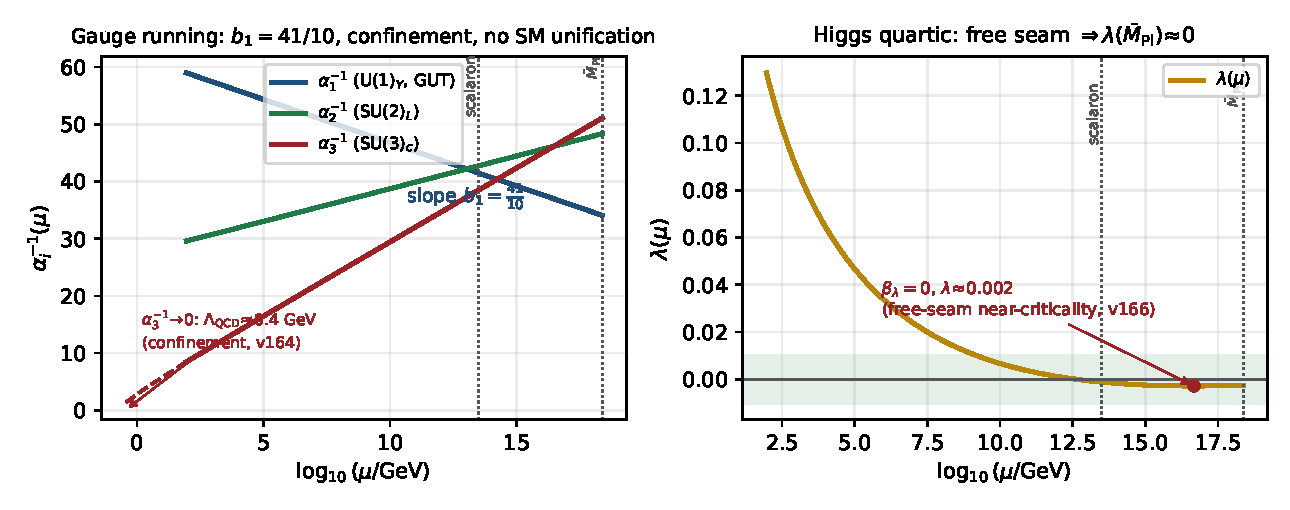
\includegraphics[width=0.98\linewidth]{figures/rg_running.pdf}
\caption{The $F_{\mathrm{transfer}}$ running (two-loop SM RGEs; the gauge $\beta$-functions
are confirmed by PyR@TE, \veri{v159\_pyrate\_gauge\_crosscheck.py}). \emph{Left:} the gauge
couplings --- the $U(1)_Y$ slope is $b_1=41/10$, $\alpha_3^{-1}\!\to\!0$ at
$\Lambda_{\mathrm{QCD}}\!\approx\!0.4$ GeV (confinement, \veri{v164\_qcd\_scale.py}), and the
Standard Model does \emph{not} unify. \emph{Right:} the Higgs quartic falls to
$\lambda(\Mpl)\!\approx\!0.002$ with $\beta_\lambda\!\approx\!0$ --- the free-seam
near-criticality that ties $m_H$ to premise~(A) (\veri{v166\_higgs\_free\_seam.py}).}
\label{fig:rg_running}
\end{figure}

% =====================================================================
\section{The Koide relation --- near $2/3$, computed exactly}
% =====================================================================
With the closed lepton source masses $\hat m_\ell\propto(\tfrac{16}{7}(\phiz)^5,\tfrac43(\phiz)^3,\tfrac76(\phiz)^2)$
the Koide ratio is a pure number (the common prefactor cancels):
\[
  Q_{\mathrm{TFPT}}=\frac{\sum_\ell \hat m_\ell}{\bigl(\sum_\ell\sqrt{\hat m_\ell}\bigr)^2}
  =0.66446\ldots,\qquad \frac23=0.66667,\qquad \text{deviation }-0.33\% .
\]
The measured pole-mass value is famously $Q_{\mathrm{PDG}}=0.66666$. So TFPT predicts a Koide ratio that
is \emph{near} $2/3$ but \emph{not exactly} $2/3$ at source level.

\begin{keybox}[Honest status of Koide \mC]
$Q_{\mathrm{TFPT}}=0.664$ is a \emph{prediction}, $0.33\%$ below $2/3$. Exact $2/3$ would require the
three carrier rationals $(\tfrac{16}{7},\tfrac43,\tfrac76)$ to satisfy a specific quadratic constraint,
which they do \emph{not}; the small residual is of the size of the source$\to$pole RG shift. We report
the near-miss honestly and do \emph{not} tune the rationals to force $2/3$.
\end{keybox}

\par\smallskip\noindent\textbf{The \emph{target} $2/3$ has a compiler reading $|\Z_2|/\Nfam$.}
The $E_8$-slice scan adds the missing piece: the value the data sits on, $Q=2/3$, is exactly
$Q_\star=|\Z_2|/\Nfam=2/3$,
the sheet over the family count --- the same two atoms $(2,3)$ that run through the whole compiler. So
the picture splits cleanly: the \emph{democratic target} is $|\Z_2|/\Nfam=2/3$ (a compiler number), and
the \emph{source-level pole-mass} value computed from the carrier rationals is $0.664$, $0.33\%$ below it
by the source$\to$pole shift. Koide is thus ``democratic $2/3$ from $(|\Z_2|,\Nfam)$, realised to
$0.33\%$ by the explicit masses'' --- promoted from a bare near-miss to a reading with a target. \mC

\par\smallskip\noindent\textbf{Conjecture: a source$\to$pole correction of size $\varphi_0/|W(A_3)|$} (\mC).
The source value sits just below $2/3$, and the deficit is almost exactly the family-Weyl quantum
$\varphi_0/|W(A_3)|$ with $|W(A_3)|=4!=24$:
\[
  Q_\ell^{\mathrm{source}}=0.6644638,\qquad
  Q_\ell^{\mathrm{source}}+\frac{\varphi_0}{24}=0.6666793,
\]
overshooting $\tfrac23=0.6666667$ by only $1.3\times10^{-5}$. So the \emph{conjecture}
$Q_\ell^{\mathrm{pole}}\approx Q_\ell^{\mathrm{source}}+\varphi_0/|W(A_3)|$ would land essentially on the
democratic $2/3$. Reported as a source$\to$pole correction \emph{conjecture}, not a derivation; the
rationals are \emph{not} tuned. \veri{v25\_frontier\_conjectures.py}

\par\smallskip\noindent\textbf{Sharper conjecture: a multiplicative seed transfer $u\to\tfrac{53}{54}u$} (\mC).
A cleaner version shifts the \emph{seed} rather than $Q$ additively, and introduces \emph{no} new free
number. Keep the lepton formula $m_e{:}m_\mu{:}m_\tau=\tfrac{16}7u^5{:}\tfrac43u^3{:}\tfrac76u^2$ but
evaluate it at the source$\to$pole seed
\[
  u_{\mathrm{pole}}^{(\ell)}=\Bigl(1-\tfrac{1}{2\Nfam^3}\Bigr)u=\tfrac{53}{54}\,u,\qquad
  54=2\cdot3^3=|\Z_2|\,\Nfam^3 .
\]
Then $Q_\ell\bigl(\tfrac{53}{54}u\bigr)=0.66666610$, i.e.\ $2/3$ to within $-5.7\times10^{-7}$ ---
an order of magnitude tighter than the additive $\varphi_0/24$ correction, with $54$ a pure compiler
number and no tuning. This sharpens the research gate to a concrete QFT task: \emph{show that the
leptonic source$\to$pole transfer of the seed is $u\mapsto u\,(1-\tfrac{1}{2\Nfam^3})$} (a renormalised-seed
effect from the leptonic self-energy or the $A_3$ family-Weyl averaging). Status remains \mC\ until that
transfer is derived. \veri{v37\_plucker\_anchor.py}

\par\smallskip\noindent\textbf{The Koide target and the QFT transfer gap are the \emph{same} quotient} (\mE/\mC).
The same $Q_\star$ controls a second, independent object --- the first non-trivial eigenvalue of the
admissible $C_6$ transport operator. Its spectrum is $\{1,(2/3)^6,(1/3)^6\}$, so
\[
  \boxed{\ \lambda_2=\Bigl(\tfrac23\Bigr)^6=Q_\star^{\,|R^+(A_3)|},\qquad Q_\star=\frac{|\Z_2|}{\Nfam},\quad |R^+(A_3)|=6\ }.
\]
The Koide democratic target, the QFT mass-gap eigenvalue $\lambda_2$ (hence $\Delta=6\log\tfrac32=-\log\lambda_2$),
and the $A_3$ positive-root hexagon are therefore \emph{one} quotient raised to one exponent. Typing:
Koide target \mC, gap eigenvalue \mE, the connection an \mE-audit. This does not ``solve'' Koide, but it
explains \emph{why} the near-value $2/3$ recurs: the same sheet-over-family ratio fixes both the
democratic lepton target and the leading transfer eigenmode.

\par\smallskip\noindent\textbf{The source$\to$pole map is \emph{forced} by that gap} (\mE/\mC).
The previous paragraph pairs the Koide target with $\lambda_2=(2/3)^6$; \vref{v82} turns the
pairing into a \emph{mechanism} (\veri{v82\_koide\_attractor\_splitting.py}). On the anchor double cover (the flavor sector) the two branch points are Koide $q=2$ and carrier
$q=5$; any branch-preserving M\"obius transfer that fixes both is, in $\rho=(q-2)/(5-q)$, exactly $\rho\mapsto\mu\rho$,
hence \emph{unique} once $\mu$ is set. Choosing $\mu=\lambda_2=(2/3)^6$ (no new number) gives the unique map
$F(q)=2(569q-3325)/(665q-3517)$ with $F'(2)=(2/3)^6<1$ and $F'(5)=(3/2)^6>1$: \textbf{Koide is the attractor, the
carrier the repeller}, and $q_n\to2$ ($x\to-2/3$) at the established gap rate. So the three structural inputs a Koide
\emph{derivation} would need collapse to \emph{one} identification --- the leptonic source$\to$pole transfer is the
branch-preserving relaxation of the gapped operator --- after which the value $2/3$, the convergence rate and the
chosen branch are all forced. This is still not a closure: that single identification stays \mC. (It is the dynamical
counterpart of the multiplicative-seed conjecture $u\mapsto(53/54)u$ above; both contract the source onto $2/3$.)

\par\smallskip\noindent\textbf{Relaxation toy: basin, exact rate, and two honest negatives} (\mE).
The relaxation picture is now stress-tested on the physical values (ledger \texttt{FR.KOIDE.05}, \veri{v93\_koide\_relaxation\_toy.py}).
\textbf{Basin lemma \mE\ (new):} under the canonical dictionary $q=\Nfam\,Q$ the \emph{entire} physical Koide
range $Q\in[\tfrac13,1]$ (Cauchy--Schwarz) maps to $q\in[1,3]$ --- the attractor $q=2$ lies inside, the
repeller $q=5$ outside: every physically possible charged-lepton configuration is in the attractor basin, no
fine-tuning of the start. \textbf{Exact rate \mE:} along the trajectory from the physical source value the
cross-ratio contracts by \emph{exactly} $(2/3)^6$ per step. \textbf{Source/pole \mE:} the exact ladder
gives $Q_{\mathrm{src}}=0.6644638$, i.e.\ $\rho_{\mathrm{src}}=-0.0021980\approx-\varphi_0/24$ to $0.8\%$ ---
the $\varphi_0/24$ conjecture re-expressed in attractor coordinates: \emph{the source sits one seed quantum
before the branch point} ($24=|W(A_3)|$); PDG pole masses give $Q_{\mathrm{pole}}=0.6666645$, the branch
point hit to $3.3\times10^{-6}$. \textbf{Honest negatives (they narrow the gate):} (i) the flow time
source$\to$pole is $t=\log_\mu(\rho_{\mathrm{pole}}/\rho_{\mathrm{src}})=2.84$ --- \emph{not} an integer, so
the literal discrete iteration $\mathrm{pole}=F^n(\mathrm{source})$ is \emph{excluded}; if the \vref{v82} map drives
the transfer at all, the missing \mC\ object is a \emph{continuous-time} generator $\exp(t\log F)$;
(ii) the $0.79\%$ mismatch of $\rho_{\mathrm{src}}$ vs $-\varphi_0/24$ is far above ladder precision, so
``exactly $\varphi_0/24$'' remains a conjecture, not an identity. The open question is no longer ``why
$2/3$?''\ but ``what is the continuous transfer generator, and why is its flow time $\sim2.8$ periods?''.

\par\smallskip\noindent\textbf{Flow time: canonical generator, data-fragility, and a conditional $m_\tau$} (\mE/\mC).
Three sharpenings of the paragraph above (ledger \texttt{FR.KOIDE.06}, \veri{v99\_koide\_flow\_time.py}); they correct the \emph{robustness} of
negative (i), not its arithmetic. \textbf{(1) The continuous generator has a canonical form \mE.} The \vref{v82}
flow is generated by the autonomous equation
\[
  \boxed{\ \frac{dq}{dt}=\frac{\Delta}{\Nfam}\,(q-2)(q-5)=\frac{\Delta}{\Nfam}\,\det B(q)\ },\qquad
  \Delta=6\log\tfrac32\ \ (\text{the gap}),
\]
whose time-$1$ map \emph{is} the M\"obius map $F$ (machine-checked; $e^{-\Delta}=(2/3)^6$ exactly). The
missing \mC\ object is therefore precisely a QFT mechanism producing \emph{gap $\times$ anchor-block
quadric} --- the form is canonical, only its physical derivation is open. \textbf{(2) The non-integrality
of $t$ is data-fragile \mE.} Because $\rho_{\mathrm{pole}}=-2.2\times10^{-6}$ sits so close to the branch
point, $t$ is hypersensitive to $m_\tau$ (PDG $1776.93\pm0.09$\,MeV): $t(-1\sigma)=2.35$,
$t(\mathrm{central})=2.84$, and $Q$ crosses $\tfrac23$ \emph{inside} the error band (at $+0.43\sigma$,
where $t\to\infty$) --- within $+0.5\sigma$, $t$ passes \emph{every} integer $\ge3$. So the exclusion of
$\mathrm{pole}=F^n(\mathrm{source})$ holds only at the central value. \textbf{(3) Conditional discrete
steps \mC\ (registry untouched; not predictions of record):} $n{=}2$ is \emph{excluded} ($-2.9\sigma$,
\mE); $n{=}3{=}\Nfam$ steps --- one per family --- predicts
\[
  \boxed{\ m_\tau=1776.9427\ \mathrm{MeV}\ }\quad(+0.14\sigma;\ \text{source-variant stable to }0.0002\ \mathrm{MeV}),
\]
while $n{=}4$ ($1776.9667$) and the exact branch ($1776.9690$) are not yet separable: the kill criterion
is $\sigma(m_\tau)\!\sim\!0.01$\,MeV (Belle~II). \emph{Look-elsewhere firewall:} a tempting scale reading
$t=\ln(M_{\mathrm{scal}}/m_\tau)/\ln W$ matched $W=46080=|W(D_5)||W(A_3)|$ to $10^{-4}$ --- and is
\emph{destroyed} by negative controls (the same hypersensitivity makes \emph{any} $W$ in a wide range land
within $0.1\sigma$); it is rejected and recorded so it is not re-fished. P2's type is unchanged (\mC, one
identification); the discrete-vs-continuous question is now \emph{experimental}, not settled.

% =====================================================================
\section{Dark matter --- the candidate is fixed, the scale is pending}
% =====================================================================
TFPT \emph{does} contain a dark-matter candidate, and it is not ad hoc: the \textbf{determinant-line
axion} of the strong-CP sector (the determinant-line axion interface of the closed branch, \mE). Two of its
inputs are already \emph{closed}:
\[
  \text{initial misalignment}\quad \theta_i=\pi\bigl(1-\varphi_{\mathrm{seam}}(\alpha_\star)\bigr)=2.974\ \text{rad}=170.4^\circ,
\]
and the domain-wall number $N_{\mathrm{DW}}$ winds once per primitive seam winding. The relic density is
the standard misalignment-plus-string expression
\[
  \Omega_a=\Omega_a^{\mathrm{mis}}(f_a,m_a,\theta_i)+\Omega_a^{\mathrm{str}}(f_a,N_{\mathrm{DW}}),
\]
and the minimal closed branch therefore has \emph{dominant axion-like dark matter}.

\par\smallskip\noindent\textbf{The $E_8$ scan rules out a rival WIMP candidate.}
The $D_8=SO(16)$ slice scan sharpens \emph{why} the axion is the candidate, not a new heavy state: the
spinor $128=(16,4)\oplus(\overline{16},\overline4)$ is the \emph{same} matter spinor as in the
$D_5\times A_3$ construction --- there is \emph{no spare $E_8$ singlet} left over to play a WIMP. Every
$E_8$ direction is accounted for by the carrier $\times$ family content. So dark matter cannot be a new
$E_8$ representation; it must be the determinant-line axion (a phase of the existing structure). A useful
\emph{negative} that removes the WIMP option on structural grounds. \mE

\begin{keybox}[Honest status of dark matter \mC/\mO]
The candidate is \emph{identified} (the axion) and its misalignment angle $\theta_i=170^\circ$ is
\emph{closed} \mE. The relic abundance still needs the decay constant $f_a$ and mass $m_a$ (interface
data set by the $M_R/\Lambda$ scales) --- a standard axion-DM computation, not yet a compiler power. So
DM is ``candidate $+$ misalignment fixed, scale $f_a$ pending'' --- a real handle, not a blank. (A
secondary candidate is the lightest seam-even sterile state near $M_R$.)
\end{keybox}

\par\smallskip\noindent\textbf{Conjecture: a determinant-line axion scale $f_a=M_{\mathrm{scal}}/128$} (\mC).
A natural compiler scale for the decay constant is the scalaron mass over the full carrier $\times$ deck
multiplicity,
\[
  f_a=\frac{M_{\mathrm{scal}}}{2\,\dim S^+\,|\mu_4|}=\frac{M_{\mathrm{scal}}}{128},\qquad
  M_{\mathrm{scal}}=\cthree^{7/2}\Mpl\approx3.06\times10^{13}\,\mathrm{GeV},
\]
giving $f_a\approx2.39\times10^{11}$ GeV and, via the standard QCD-axion relation
$m_a\simeq5.70\,\mu\mathrm{eV}\,(10^{12}\,\mathrm{GeV}/f_a)$, a mass $m_a\approx23.8\,\mu\mathrm{eV}$.
This is consistent with the closed near-hilltop misalignment $\theta_i=170.4^\circ$, but it is a
\emph{cosmological scenario} (sensitive to anharmonic / string corrections near the hilltop), not a closed
hit. \veri{v25\_frontier\_conjectures.py}

% =====================================================================
\section{Full quantum gravity --- induced from the boundary kernel}
% =====================================================================
\emph{Framing (read this first):} full QG closure is a \textbf{certification layer}, not a prerequisite.
TFPT does \emph{not} need the complete quantum-gravity measure to test its Standard-Model and cosmology
readouts --- those run through $v_{\mathrm{geo}}$ and $F_{\mathrm{transfer}}$ and are falsifiable now
(JUNO, CMB-S4, EDM). $G_{\mathrm{net}}$ certifies the metric sector; its absence narrows what can be
\emph{claimed}, not what can be \emph{tested}.
\smallskip\\
The normalisation $\cthree=1/(8\pi)$ \emph{is} the gravitational seam constant: in TFPT gravity is
\emph{induced} from the boundary kernel (P1), not separately quantised. The $R^2$/scalaron sector
(question 2) is the low-curvature effective theory; the \emph{full} theory is the boundary-kernel measure.
\emph{Newton's constant is then not an \emph{independent} input:} fixing the physical $\Lambda$ branch
($(8\pi)^2\delta_{\mathrm{top}}=\tfrac{3}{4\pi^2}$) pins $\bar M_{\mathrm{Pl}}$ \emph{relative to} $\Lambda$, so
$G_N$ is read out \emph{after} selecting the physical $\Lambda$ branch \emph{and} fixing the one dimensionful
induced-gravity (Sakharov) anchor (\mE/\mC, \veri{v60\_lambda\_metrology\_branch.py}) --- a metrology readout,
not a from-nothing prediction.

\begin{center}
\begin{tikzpicture}[font=\footnotesize,
  b/.style={rectangle,rounded corners,draw,thick,align=center,inner sep=3pt,minimum height=8mm},
  ar/.style={-{Stealth[length=2mm]},thick,gray}]
  \node[b,draw=tfred!80!black,fill=tfred!8] (p1) at (0,0) {boundary kernel (P1)\\$\cthree=\tfrac1{8\pi}$};
  \node[b,draw=tfgreen!70!black,fill=tfgreen!8] (r2) at (3.9,0) {induced $R+R^2$\\(low curvature)};
  \node[b,draw=tfblue,fill=tfblue!8] (os) at (8.0,0) {boundary-kernel measure\\$=$ full quantum gravity};
  \draw[ar] (p1)--(r2); \draw[ar] (r2)--(os);
  \draw[ar,dashed] (p1) to[bend right=22] node[below,font=\scriptsize]{induces} (os);
\end{tikzpicture}
\end{center}

\begin{keybox}[Honest status of quantum gravity --- physical sector closed, ambient gap-decoupled \mE/\mO]
``Full quantum gravity beyond the $R^2$ sector'' is, in TFPT, \emph{not} a separate graviton-quantisation
programme: it is the well-definedness of the \emph{boundary-kernel path-integral measure} extended to the
dynamical metric beyond the FRW/minisuperspace reduction. Two results sharpen its status.
\textbf{(i) Heat-kernel grounded (G2).} The spectral action $\operatorname{Tr}f(D/\Lambda)$ gives, via the
standard Seeley--DeWitt coefficients for the Dirac operator ($a_2\!\sim\!-R/3$, $a_4|_{R^2}\!\sim\!R^2/72$),
Einstein--Hilbert $+$ $R^2$ \emph{structurally} --- the $R+R^2$ form is not postulated; the scalaron ratio
$M^2/\Mpl^2=6(4\pi)^2/f_0$ with the TFPT closure $\cthree^7$ fixing the cutoff moment $f_0$.
\textbf{(ii) Gap-decoupled (G5).} The metric coupling is gap-dominated,
$2\|V_{\mathrm{metric}}\|=0.785<\Delta=6\log\tfrac32=2.433$, so the admissible sector keeps a strictly
positive effective gap $\Delta_{\mathrm{eff}}=1.648>0$ under the stated RP and metric-coupling assumptions.
A positive gap protects the admissible IR sector from the un-built ambient, so under those assumptions the
admissible-sector measure is closed. \textbf{What remains \mO:} the ambient metric measure --- the
projective limit (G6) --- is the $G_{\mathrm{metric}}$ research gate; we do \emph{not} claim it is
physically irrelevant (that would itself be a physical interpretation), only that it is decoupled from the
admissible IR sector under the stated assumptions. \veri{v36\_spectral\_action\_g2.py}
\smallskip\\
\noindent\emph{Update (QBL chain, \vref{v108}--\vref{v113}):} the boundary-net residual now carries \emph{double}
weight --- the carrier choice $g=5$ has been reduced to the \emph{same} premise. The certified scalar
kernel exists iff it pairs the two sheets, the certified channel counts the code identically (Pascal
closure $=$ channel identity), pair transport is minimally complete, and the single quasi-free kernel
(rank $=c$: $5$ carrier block, $8$ seam hull) is the defining datum of the free $c=8$ net this gate
already posits. Closing the index-$4$ statement therefore also closes the carrier selection \mE\
(see \texttt{tfpt\_1} and \texttt{tfpt\_research\_contracts}). \veri{v113\_quasifree\_kernel.py}
\smallskip\\
\noindent\emph{Update (free-bulk premise discharged, \vref{v160}--\vref{v165}):} that ``free $c{=}8$ net''
premise is no longer free-standing. It is a fixed-point theorem (quasi-free $\Rightarrow$ all higher
cumulants $\kappa_{2n}{=}0$, \vref{v160}); the infinite Schwinger cone is \emph{eliminated} --- by
Bogoliubov second quantisation the cone gap equals the one-particle gap $(2/3)^6$ (\vref{v161}), forced by
$\mu_4$-equivariance (\vref{v162}); and the residual factors into the already-open $A_2$ net-existence (an
assembly of established net constructions, \mC) and $R_1=$ \texttt{GATE.QGEO}, with the irreducible core
$\{\pi,v_{\mathrm{geo}}\}$ a theorem (\vref{v165}). So the metric-sector gate carries \emph{zero new}
independent open content. \veri{v165\_premise\_a\_closure.py}
\end{keybox}

% =====================================================================
\section*{Summary}
% =====================================================================
\addcontentsline{toc}{section}{Summary}
\begin{center}\small
\renewcommand{\arraystretch}{1.25}
\begin{tabularx}{\linewidth}{@{}p{2.9cm}cY@{}}
\toprule
\textbf{Item} & \textbf{Status} & \textbf{Honest handle / what is missing} \\
\midrule
$\eta_B$ & \mC & downstream readout $=6.1{\times}10^{-10}$ from closed $\Omega_b h^2$; leptogenesis is an interface (Boltzmann) \\
$m_p/m_e$ & \mO & cross-sector (QCD scale / closed $m_e$); scheme-level, not a compiler power \\
Koide $Q$ & \mC & computed $Q=0.664$, $0.33\%$ from $2/3$; near, not exact --- not tuned \\
dark matter & \mC/\mO & determinant-line axion candidate fixed, $\theta_i=170^\circ$ closed; relic scale $f_a,m_a$ open \\
quantum gravity & \mE/\mO & $R+R^2$ heat-kernel grounded (G2); physical sector gap-decoupled; only ambient limit (G6) open \\
\bottomrule
\end{tabularx}
\end{center}
\markerkey

\noindent\textbf{Net (honest).} Two of the five have a genuine quantitative handle that already lands on
the data ($\eta_B=6.1\times10^{-10}$ via the closed $\Omega_b$; the axion DM candidate with a closed
misalignment angle). One is a computed \emph{near}-miss reported without tuning (Koide $0.664$ vs $2/3$).
One is structural-only and left open ($m_p/m_e$ as a cross-sector ratio); quantum gravity has been
sharpened --- its $R+R^2$ form is now heat-kernel grounded (G2) and its physical sector is gap-decoupled
(G5), leaving only the ambient projective limit (G6) as a mathematical-completeness item. None has been
forced onto the compiler ladder --- which is exactly the right call: the strong results stay strong
precisely because the weak ones are not oversold.

% =====================================================================
\section*{Appendix: computational verification}
\addcontentsline{toc}{section}{Appendix: computational verification}
% =====================================================================
These are the \emph{frontier} items: most carry \mO\ (open) or \mC\ (conditional) and are therefore
\emph{not} part of the pass/fail suite. The one quantitative handle that is reproduced is
$\Omega_b{=}(1{-}\tfrac1{4\pi})\phiz$ (whence the $\eta_B$ order) in
\texttt{verification/v7\_gravity\_cosmo.py}. The $R+R^2$ structure and the gap-decoupling of the physical
QG sector \emph{are} machine-checked (\texttt{v28\_gravity\_fR.py}, \texttt{v36\_spectral\_action\_g2.py});
only the proton/electron ratio and the ambient projective limit (G6) are left open by design --- no script
``proves'' those, consistent with their \mO\ marking. The compiler/SM
identities they build on are checked by the suite in \texttt{verification/} (run
\texttt{python verification/run\_all.py}; see \texttt{verification/README.md}).

\end{document}
